\chapter{Implementazione}
\label{ch:implementazione}

\section{Tecnologie utilizzate}
Il prototipo è realizzato in \Erlang{}\footnote{\url{http://www.erlang.org/}} e \Python{}\footnote{\url{http://www.python.org/}} con l'utilizzo delle librerie \textsl{TwOTP}\footnote{\url{http://launchpad.net/twotp}} e \textsl{Qt}\footnote{\url{http://qt.nokia.com/}} usate rispettivamente per l'implementazione del protocollo di distribuzione \Erlang{} su nodi \Python{} e per la costruzione di GUI con il supporto dei \textit{bindings} \textsl{PyQt}\footnote{\url{http://www.riverbankcomputing.co.uk/software/pyqt/intro}}.

Di seguito le versioni del software utilizzato:
\begin{center}
\begin{tabular}{c|c}
\textbf{Software} & \textbf{Versione testata} \\
\hline
Erlang & R13B04 o successiva \\
\hline
Python & 2.6.4 \\
\hline
Twisted & 9.0.0 o successiva \\
TwOTP & 0.7 \\
\hline
Qt & 4.6.x \\
PyQt & 4.7.3 o successiva \\
\end{tabular}
\end{center}

Il criterio su cui ci siamo basati per decidere in quale linguaggio implementare una componente è abbastanza semplice: se la componente comprende un'interfaccia grafica utilizzare \Python{} più le librerie sopra citate, \Erlang{} altrimenti. Risulta dunque la seguente suddivisione:
\begin{center}
\begin{tabular}{|p{0.2\textwidth}|p{0.3\textwidth}|}
\hline
\multirow{6}{*}{\textbf{Erlang}} & \sched{}\\
& \evdisp{}\\
& \track{}\\
& \team{}\\
& \car{}\\
& \weather{}\\
\hline
\multirow{4}{*}{\textbf{Python}} & \texttt{race\_info}\\
& \texttt{debug\_log}\\
& \texttt{team\_monitor}\\
& \texttt{weather\_station}\\
\hline
\end{tabular}
\end{center}

\subsection*{Caratteristiche di Erlang}
\Erlang{} è un linguaggio di programmazione funzionale \textit{general-purpose} con \textit{dynamic typing} e supporto nativo per concorrenza e distribuzione. Per recuperare parte dei controlli statici sul codice abbiamo deciso di utilizzare anche \textsl{Dialyzer}, uno strumento di analisi statica per \Erlang{}.

Le caratteristiche del linguaggio che incidono particolarmente sul progetto sono l'assenza di memoria condivisa e la modalità di comunicazione tra processi (scambio di messaggi asincrono).
Per informazioni più dettagliate sul linguaggio fare riferimento alla documentazione consultabile all'indirizzo \url{http://www.erlang.org/doc/getting_started/conc_prog.html}.

Una singola istanza di una macchina virtuale \Erlang{} è detta anche nodo \Erlang{} e un sistema \Erlang{} distribuito è composto quindi da una rete di tali nodi. Il protocollo di distribuzione usato nel progetto è il protocollo di distribuzione \Erlang{} che permette la comunicazione tra due nodi \Erlang{} grazie anche a EPMD (\textsl{Erlang Port Mapper Daemon}) avviato automaticamente al bootstrap di ogni nodo.

Una delle caratteristiche più apprezzabili e utili di questo linguaggio è che i processi residenti su nodi differenti comunicano tra di loro esattamente allo stesso modo in cui comunicano due processi sullo stesso nodo. Questa caratteristica permette di passare facilmente dal concorrente al distribuito e viceversa, in modo trasparente al programmatore.

\subsection*{Mnesia}
\textsl{Mnesia}\footnote{\url{http://www.erlang.org/doc/apps/mnesia/users_guide.html}} è un database distribuito per \Erlang{} che supporta sia copie RAM che copie persistenti e permette di salvare strutture dati complesse a piacere. Nel prototipo è stato utilizzato principalmente nella componente \track{} per salvare dati relativi allo stato della pista e in generale per la memorizzazione di impostazioni di configurazione relative alla singola competizione.

Il linguaggio usato per le query è \Erlang{} stesso, differentemente da quanto avviene per altri linguaggi e DBMS, e questo rende decisamente più omogeneo e leggibile il codice. Ovviamente \textsl{Mnesia} supporta le transazioni e per di più in un modo molto semplice da usare e che sfrutta a pieno la natura funzionale del linguaggio. L'esecuzione di una transazione avviene infatti grazie alla chiamata \fun{mnesia:transaction(F)} dove F è la funzione che contiene le istruzioni da eseguire in modo atomico.

\subsection*{Interazione Erlang $\leftrightarrow$ Python: TwOTP}
\textsl{TwOTP} (\textit{Twisted interface to Erlang/OTP}) è una libreria che implementa il protocollo di distribuzione \Erlang{} in linguaggio \Python{} con l'ausilio di \textsl{Twisted}.

\textsl{Twisted}\footnote{\url{http://twistedmatrix.com/}} è un framework per sviluppare applicazioni che interagiscono con la rete fornendo al programmatore un solido e flessibile \textit{networking engine} asincrono basato su eventi e \textit{callbacks}.

\section{Avvio del sistema}
\label{sec:avvio}
Il diagramma di comunicazione in figura~\ref{fig:bootstrap} rappresenta la sequenza di \textit{bootstrap} del sistema. \texttt{control\_panel} e \texttt{node\_configurator} sono avviati dall'utente su elaboratori in rete tra loro e senza un ordine predefinito. Le componenti grafiche provvedono a generare un nome casuale e lo usano nell'istanziare un nodo \Erlang{} sullo stesso elaboratore.

Nel nodo \Erlang{} istanziato da \texttt{control\_panel} viene eseguito \bootserv{} attraverso la chiamata \fun{start}, mentre sui nodi istanziati da \texttt{node\_configurator} vengono istanziati processi \nodeman{}. Durante l'avvio di \nodeman{} viene consultato il file \texttt{.hosts.erlang} che contiene i nomi degli \textit{hosts} che possono prendere parte alla simulazione e permette di identificare tali nodi sulla rete.
Tramite \texttt{control\_panel} l'utente deve indicare:
\begin{itemize}
\item percorso dei file di configurazione,
\item numero di giri della simulazione,
\item fattore di \textit{simulation speed} iniziale.
\end{itemize}
Tramite \texttt{node\_configurator} bisogna invece indicare il numero di componenti necessarie alla simulazione che possono essere istanziate su quel nodo. Le componenti disponibili sono: \sched{}, \evdisp{}, \car{}, \team{}, \weather{}.

Una volta che queste informazioni sono state inserite, esse vengono comunicate alle rispettive componenti \Erlang{} con l'invocazione a \fun{read\_config\_files} e \fun{configure}. Effettuando il \textit{parsing} dei file di configurazione, la logica di \fun{read\_config\_files} è in grado di calcolare la richiesta di risorse di simulazione necessarie, mentre \fun{node\_manager:configure}, con il metodo \fun{add\_node} comunica a \bootserv{} le disponibilità di risorse di quel nodo. Una volta raggiunta la quota necessaria di risorse viene inviato il messaggio \fun{ready} a \texttt{control\_panel} che può quindi abilitare il pulsante di \textit{bootstrap}.

A questo punto l'utente può interagire con l'interfaccia grafica e causare l'invocazione del metodo \fun{bootstrap\_server:bootstrap} che provvede a inizializzare \textsl{Mnesia} e creare le tabelle vuote che verranno successivamente utilizzate dal sistema. Grazie alle informazioni di configurazione viene anche generata la tabella contenente la descrizione della pista. Successivamente il metodo \fun{bootstrap} istanzia, attraverso \fun{node\_manager:start\_app}, tutte le componenti di simulazione necessarie, nell'ordine:
\begin{enumerate}
\item \evdisp{}
\item \sched{}
\item \weather{}
\item \team{}
\item \car{}
\end{enumerate}
Poiché sussistono delle dipendenze tra le varie componenti, \bootserv{} attende che l'inizializzazione di un'applicazione sia completa prima di procedere con l'avvio delle applicazioni che dipendono da essa. Istanze diverse di una stessa componente vengono invece avviate in parallelo, dato che non vi può essere alcuna dipendenza tra loro, sia che si trovino sullo stesso nodo, sia che si trovino su nodi differenti.

\begin{landscape}
\begin{figure}
\begin{center}
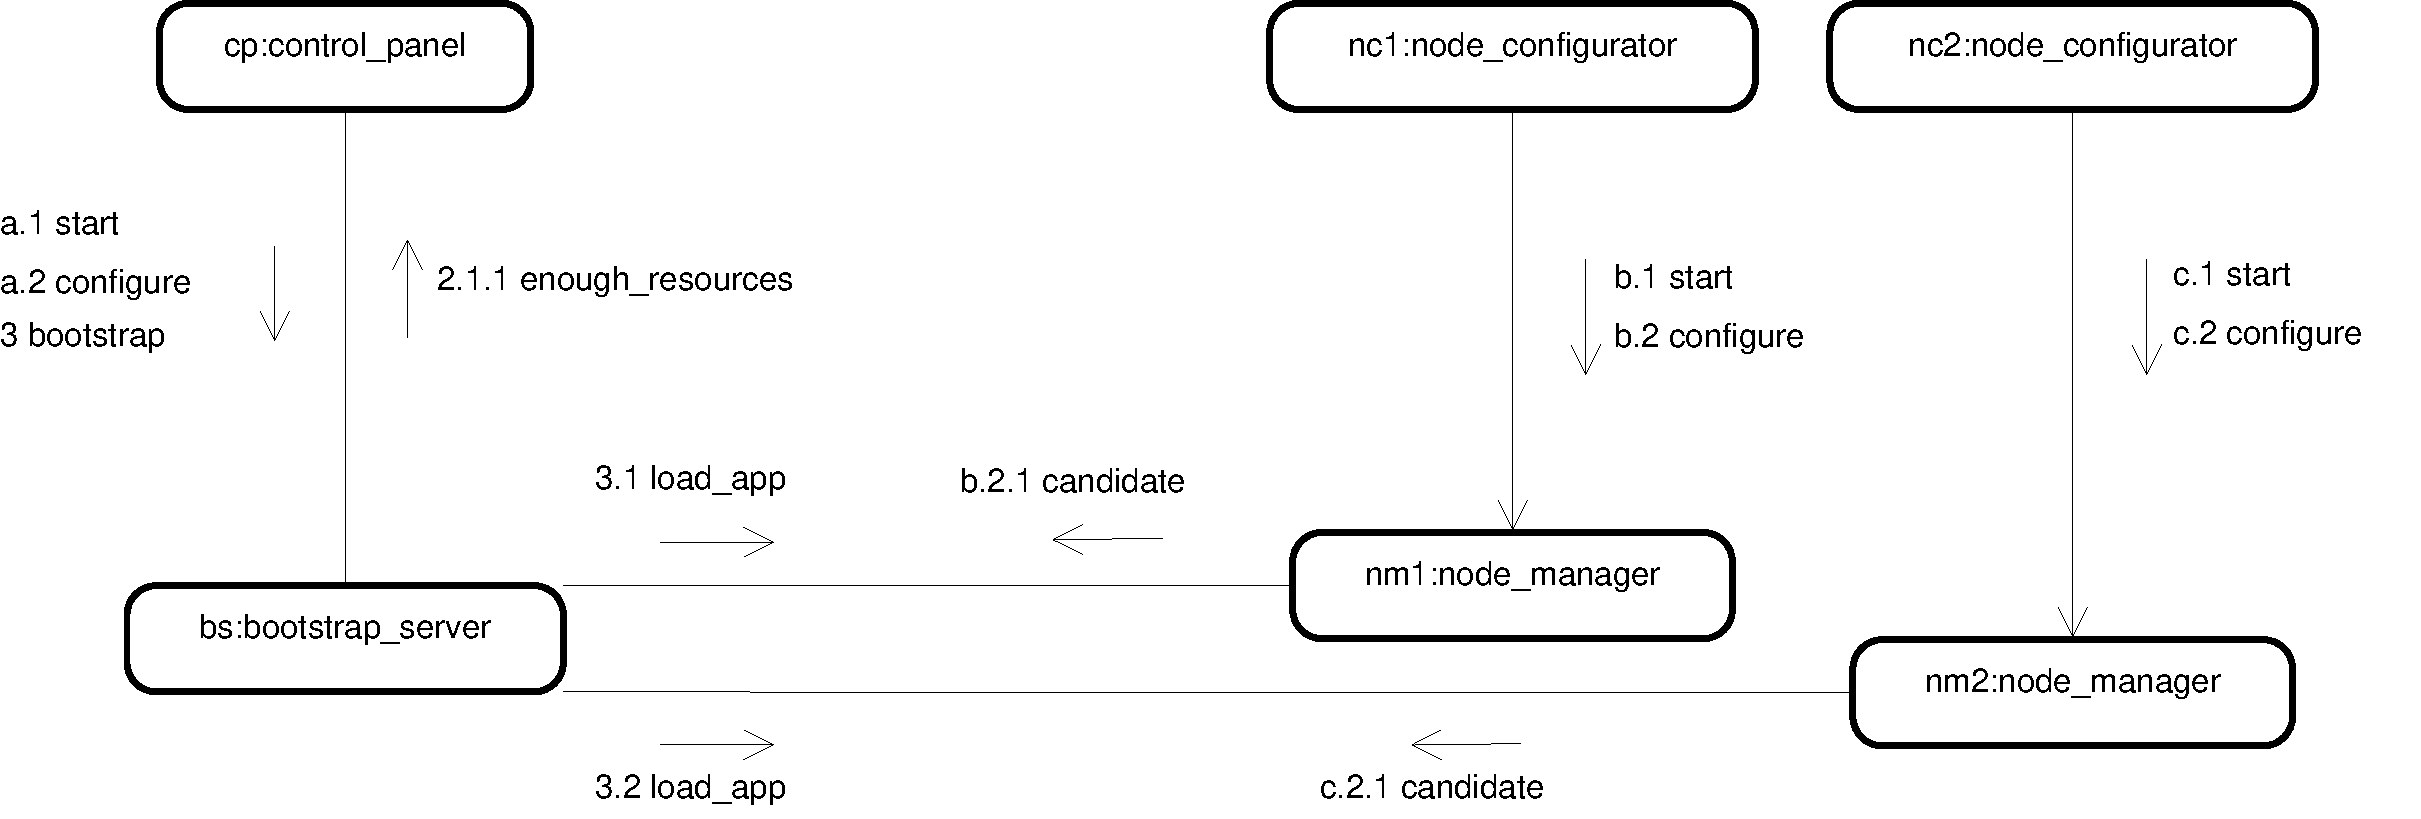
\includegraphics[height=.25\paperheight]{diagrammi/Bootstrap}
\caption{Diagramma della fase di \textit{bootstrap}}
\label{fig:bootstrap}
\end{center}
\end{figure}
\end{landscape}

\section{Dinamiche della competizione}
\subsection{Partenza}
\label{sec:partenza}
Prima che l'utente possa dare il via alla competizione tutte le auto devono essersi registrate presso lo \sched{} indicando come tempo di prenotazione $0$. \`E importante precisare che, in questa situazione, l'ordine in cui lo \sched{} permette ai processi \car{} di andare in esecuzione non influenza l'esito della gara: infatti alla partenza le auto sono tutte su segmenti diversi e di conseguenza non concorrono tra di loro per l'accesso ad uno stesso segmento. Ne deriva quindi che sebbene l'ordine di esecuzione alla partenza possa essere considerato casuale (dipende dall'ordine di registrazione presso lo \sched{}, che è una componente distribuita del sistema), questo non va ad influenzare i tempi di percorrenza dei segmenti da parte delle auto e non influisce quindi con il risultato della gara.
La disposizione iniziale delle auto sulla pista avviene similmente a quanto riportato in figura~\ref{fig:startGrid}, ed è richiesto all'utente che nella zona di pista che precede la linea di arrivo vi siano almeno tre corsie.

\begin{figure}
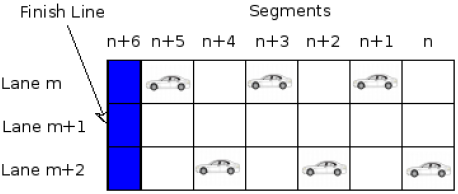
\includegraphics[width=\textwidth]{diagrammi/StartGrid}
\caption{Griglia di partenza}
\label{fig:startGrid}
\end{figure}

\subsection{Percorrenza di un segmento}
\label{sec:percorrenza}
Nel momento in cui un'auto si appresta a percorrere un segmento sono noti alla componente \fun{track}:
\begin{itemize}
\item corsia di ingresso,
\item velocità di ingresso,
\item tempo di ingresso,
\item conformazione e stato del segmento,
\item caratteristiche e stato dell'auto,
\item informazioni su altre auto che stanno percorrendo quel segmento.
\end{itemize}

Grazie alle informazioni sopra elencate e indicando in quale corsia il pilota vuole trovarsi all'uscita del segmento è possibile calcolare il tempo e la velocità di uscita dell'auto. Sono principalmente due i gruppi di fattori che influenzano questo calcolo: in primo luogo l'auto stessa e le caratteristiche della pista, poi la presenza di altre auto nello stesso segmento e l'interazione con esse.

Iniziando ad analizzare il primo gruppo di fattori risulta evidente che vi è una velocità massima che un'auto può mantenere in un segmento per evitare di uscire di pista, in particolare nei segmenti curvilinei la forza di attrito deve essere sufficiente a contrastare la forza centrifuga.
Visto che la forza d'attrito dipende anche dalle caratteristiche e dallo stato dell'auto, ne consegue che tale velocità massima può essere diversa per ogni auto.
Un altro vincolo alla velocità è dato dal regolamento di gara per quanto riguarda la percorrenza della \textit{pit lane}, tuttavia questo vincolo non riguarda l'intero segmento ma solo una determinata corsia e va applicato solo sulle auto che stanno per rientrare ai \textit{box} per effettuare una sosta.

I segmenti appena considerati non sono tuttavia gli unici ad avere un limite alla velocità alla quale possono essere percorsi. Basta pensare alle azioni che i piloti effettuano prima di intraprendere una curva nella realtà per capire che un segmento curvilineo impone vincoli alla velocità di percorrenza anche nei segmenti che lo precedono. \`E quindi corretto affermare che ogni segmento della pista ha un limite di velocità, sia esso diretto o indiretto.

Inoltre il numero di segmenti che impone limiti di velocità diretti può cambiare in base al fatto che il pilota voglia o meno effettuare una sosta ai \textit{box}. Di conseguenza cambieranno anche i limiti indiretti. Per questo motivo abbiamo deciso di modellare questo fatto associando ad ogni segmento due limiti di velocità, aggiornati dinamicamente nel corso della competizione: uno da rispettare nel caso in quel giro non si voglia effettuare una sosta ai box, l'altro nel caso opposto. In caso di sosta ai box è necessario infatti che la vettura mantenga, in prossimità dell'ingresso alla \textit{pitlane}, una velocità sufficientemente bassa da permettere di rallentare prima di effettuare l'ingresso nella zona sottoposta a limite di velocità dal regolamento.

La fase in cui vengono calcolati i due limiti di velocità per ogni segmento della pista è detta ``fase di preelaborazione'' e viene effettuata da ciascuna auto:
\begin{enumerate}
\item all'inizio della gara;
\item ogni volta che passa per il traguardo;
\item dopo ogni sosta ai \textit{box};
\item dopo ogni cambio delle condizioni atmosferiche.
\end{enumerate}
Il calcolo al punto 1 avviene poiché non è possibile per un'auto effettuare una mossa senza avere una tabella di preelaborazione, al punto 2 per avere una stima più accurata dei valori necessari che consideri il livello di carburante e usura pneumatici attuale e ai punti 3 e 4 poiché in corrispondenza di tali eventi può cambiare di molto l'attrito pneumatici/pista e invalidare quindi la preelaborazione precedente.

Nel calcolo dei limiti di velocità indiretti è molto importante la decelerazione massima che un'auto può raggiungere: per rendere la simulazione più verosimile abbiamo deciso di trattare in modo abbastanza dettagliato la parte fisica della competizione, facendo dipendere accelerazione e decelerazione massime sia dalle caratteristiche dell'auto che da quelle della pista.
In particolare l'accelerazione/decelerazione che un auto può erogare in un determinato segmento dipende da:
\begin{itemize}
\item potenza del motore/dei freni,
\item peso dell'auto a secco,
\item peso del pilota,
\item peso del carburante,
\item stato di usura e tipo dei pneumatici,
\item condizioni atmosferiche,
\item inclinazione della pista.
\end{itemize}

\begin{figure}
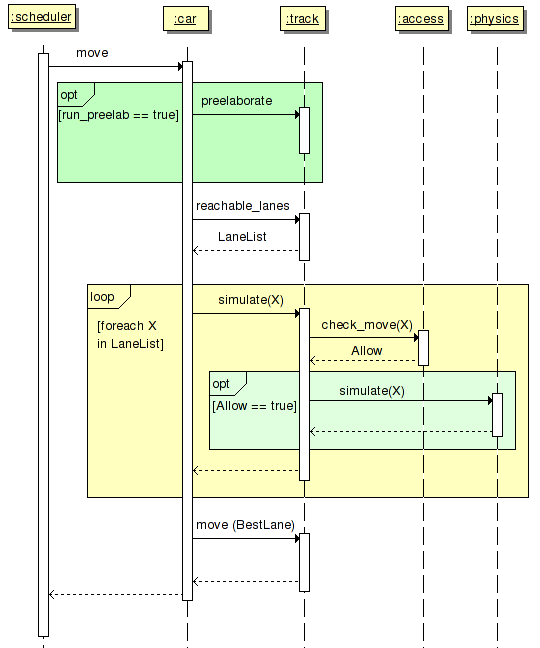
\includegraphics[width=\textwidth]{diagrammi/Simulation}
\caption{Fase di simulazione}
\label{fig:simulation}
\end{figure}

Passiamo ora a descrivere le operazioni che il processo \car{} effettua nel momento in cui lo \sched{} gli consente di eseguire una mossa.

Dal punto di vista del processo \car{} la sequenza di invocazioni necessaria per effettuare uno spostamento sulla pista è indipendente sia dalla posizione dell'auto che dalla conformazione della pista stessa.

Restando ad alto livello, il protocollo di interazione tra \car{} e \track{} è il seguente: per percorrere il segmento successivo, la componente \car{} prima utilizza il metodo \texttt{track:simulate} per ottenere i dati necessari a scegliere quale sia la corsia più conveniente e successivamente invoca il metodo \texttt{track:move} per effettuare lo spostamento.
Grazie a questo schema le componenti \car{} non devono essere a conoscenza della conformazione della pista per poterla percorrere in quanto i segmenti vengono trattati tutti in modo omogeneo.

In altre parole è la componente \track{} che si occupa di individuare il segmento che l'auto dovrà percorrere e più in generale di gestire l'accesso ai segmenti. In base al tipo di segmento \track{} provvederà ad effettuare tutte le operazioni del caso (rilevazioni cronometriche, comunicazione con la relativa componente \team{} in caso di sosta ai box, ecc\ldots) nascondendo quindi le differenze tra i vari tipi di segmenti alla componente \car{}.

Un altra conseguenza della soluzione adottata è che non è necessario che un'auto conosca esplicitamente la posizione sulla pista degli altri concorrenti, in quanto questo aspetto viene gestito da \track{}.


Come si può vedere in figura~\ref{fig:simulation}, la prima operazione è l'eventuale ricalcolo della tabella di preelaborazione; successivamente viene controllato se è prevista una sosta ai \textit{box} per il giro corrente; infine si passa alla fase di simulazione vera e propria. Nella fase di simulazione \car{} richiede a \track{} quali sono le corsie raggiungibili nel segmento che sta per percorrere e successivamente di simulare l'esito dello spostamento per ogni corsia che l'auto può raggiungere. Questa fase, implementata da \fun{track:simulate}, può restituire diversi risultati a \car{}.
\begin{itemize}
\item \texttt{race\_ended}: l'auto nella mossa precedente ha superato il traguardo nell'ultimo giro e ha quindi terminato la sua gara.
\item \texttt{fail}: l'auto non può effettuare la mossa richiesta a causa di uno dei seguenti motivi:
        \begin{itemize}
        \item il carburante è esaurito;
        \item i pneumatici sono esplosi per l'eccessiva usura;
        \item la scuderia ha ordinato il ritiro dell'auto dalla competizione;
        \item non è possibile occupare la corsia richiesta poiché il regolamento lo vieta;
        \item si sta cercando di entrare nella \textit{pit lane} senza aver segnalato la sosta;
        \item la corsia che si vuole percorrere è già occupata e la capacità di frenata non è sufficiente ad accodarsi all'auto che precede;
        \item l'auto non è in grado di mantenersi in pista a causa della velocità eccessiva.
        \end{itemize}
\item \texttt{pits}: l'auto effettuerà una sosta ai \textit{box}.
\item \texttt{Time}: il tempo in cui l'auto uscirà da quel segmento calcolato come tempo di ingresso più tempo di percorrenza.
\end{itemize}
Una volta ottenuti i risultati della simulazione, la logica di \car{} decide quale sia la corsia migliore da percorrere, in particolare l'auto sceglierà la corsia la cui simulazione ritorna il valore (in ordine di priorità decrescente):
\begin{enumerate}
\item \texttt{race\_ended};
\item \texttt{pits};
\item il valore \texttt{Time} minore;
\item \texttt{fail}.
\end{enumerate}

\begin{figure}
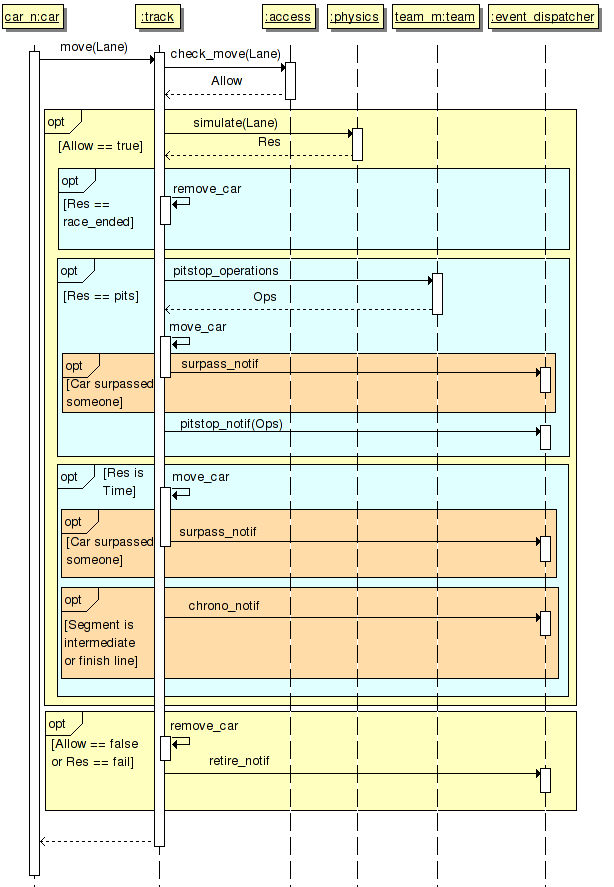
\includegraphics[width=\textwidth]{diagrammi/Move}
\caption{Fase di spostamento}
\label{fig:move}
\end{figure}

Una volta scelta la corsia migliore \car{} effettua lo spostamento sulla pista grazie all'invocazione \fun{track:move} (figura~\ref{fig:move}) e resta in attesa del risultato che può essere o il tempo di uscita dal segmento che si sta percorrendo oppure \texttt{race\_ended} oppure \texttt{fail}. Nel primo caso l'auto provvederà a prenotarsi presso lo \sched{} indicando il tempo di uscita, negli altri casi \car{} non effettuerà alcuna nuova prenotazione.

La prima parte della fase di spostamento è molto simile alla fase di simulazione poiché viene controllato se la mossa è consentita o meno e viene eventualmente calcolato il tempo di uscita dal segmento anche nel caso in cui si tratti di una sosta ai \textit{box}.

Un fatto importante da notare è che una mossa è ritenuta non consentita dalla funzione \texttt{move} se e solo se l'invocazione del metodo \texttt{simulate} effettuata con gli stessi parametri ha come valore di ritorno \texttt{fail}.
Di conseguenza nel momento in cui \car{} va ad invocare \texttt{track:move} con parametri relativi ad una mossa non consentita, visto il criterio di scelta utilizzato per la corsia di uscita precedentemente descritto, siamo certi che non esistevano mosse consentite e che tutte le invocazioni del metodo \texttt{track:simulate}, effettuate nella precedente fase di simulazione, hanno avuto come esito \texttt{fail}.

Nella seconda parte dello spostamento vengono emesse eventuali notifiche verso \evdisp{}.

Il metodo \fun{move\_car} è particolarmente importante ai fini della simulazione poiché serve a individuare eventuali sorpassi avvenuti all'interno del segmento e notificarli. Un ulteriore compito del suddetto metodo è quello di aggiornare lo stato di \track{} contenuto nel \textit{database}.

Il metodo \fun{move\_car} deve anche calcolare i consumi dell'auto derivanti dall'aver percorso quel segmento.
Il consumo di carburante è pari a una quantità fissa per segmento moltiplicata per un coefficiente dipendente dall'inclinazione della pista in quel punto, mentre il consumo dei pneumatici dipende dalla curvatura del segmento, dal tipo di pneumatici usati e dalle condizioni atmosferiche.

\subsection{Intermedi cronometrici}
Gli intermedi cronometrici e il traguardo sono particolari segmenti aventi lunghezza nulla. Dal punto di vista di \car{} sono trattati esattamente come tutti gli altri segmenti in quanto è compito di \track{} nascondere le differenze ed effettuare semplificazioni dove possibile. Avendo lunghezza zero, non è necessario effettuare il calcolo del tempo di percorrenza. Infatti per questo tipo di segmenti, detti:
\begin{itemize}
\item $n+1$: l'indice di tale segmento;
\item $L_{ex_A}^{n}$: la corsia di uscita di A dal segmento $n$;
\item $L_{ex_A}^{n+1}$: la corsia di uscita di A dal segmento $n+1$;
\item $T_{en_A}^{n+1}$: il tempo di ingresso di A nel segmento $n+1$;
\item $T_{ex_A}^{n}$: il tempo di uscita di A dal segmento $n$;
\item $T_{ex_A}^{n+1}$: il tempo di uscita di A dal segmento $n+1$;
\end{itemize}
allora valgono:
\begin{itemize}
\item $L_{ex_A}^{n} = L_{ex_A}^{n+1}$: imposto dal modulo \texttt{access} poiché non è possibile cambiare corsia in un segmento di lunghezza nulla;
\item $T_{ex_A}^{n} = T_{en_A}^{n+1} = T_{ex_A}^{n+1}$: poiché il tempo impiegato a percorrere un tratto di lunghezza nulla è nullo;
\item la velocità di uscita dal segmento $n+1$ è uguale alla velocità di ingresso nel medesimo segmento;
\item non possono avvenire sorpassi all'interno di tale segmento;
\item il percorrere tale segmento non causa consumo né di carburante né di pneumatici.
\end{itemize}
Come si può notare in figura~\ref{fig:move} in corrispondenza del transito di un'auto attraverso un intermedio cronometrico viene emessa da \track{} una \texttt{chrono\_notif} verso \evdisp{}. Questo tipo di messaggio contiene:
\begin{itemize}
\item ID dell'auto;
\item ID dell'intermedio e numero del giro;
\item tempo di gara in cui l'auto attraversa l'intermedio;
\item velocità massima raggiunta dall'auto dopo l'intermedio precedente;
\item stato corrente di carburante e pneumatici dell'auto.
\end{itemize}

\subsection{Pit lane}
\begin{figure}
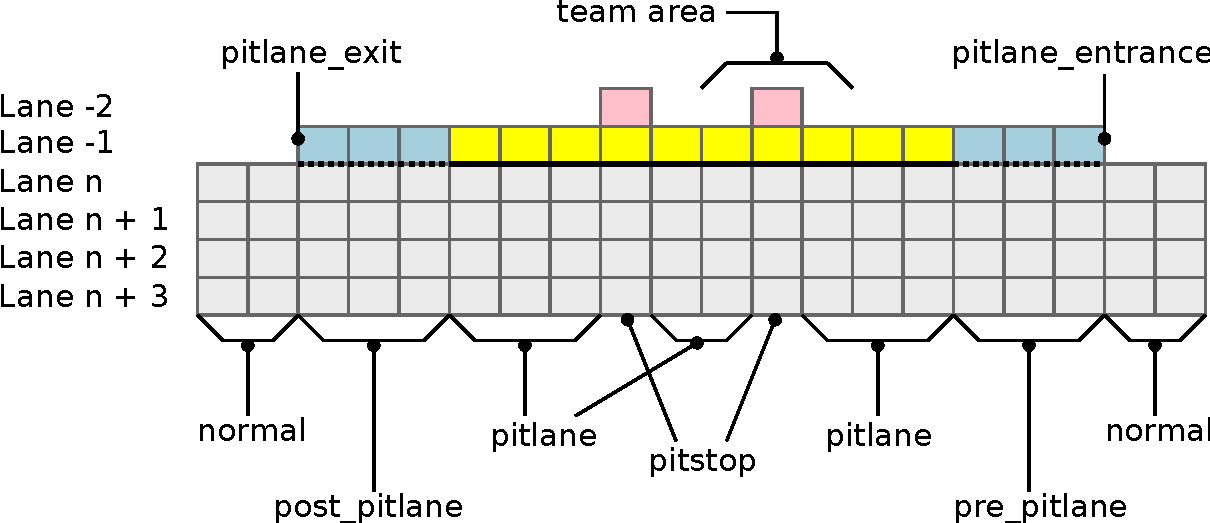
\includegraphics[width=\textwidth]{diagrammi/PitLane}
\caption{Rappresentazione della zona dei \textit{box}}
\label{fig:pitLane}
\end{figure}

La sezione di pista indicata dall'utente come zona \textit{box} (attraverso l'impostazione di \texttt{pitlane\_entrance} e \texttt{pitlane\_exit} nel file di configurazione) viene rappresentata dalla componente \track{} come mostra la figura~\ref{fig:pitLane}. Le corsie con indice maggiore o uguale a $n$ sono quelle indicate dall'utente nel file di configurazione mentre le corsie $-1$ e $-2$ sono generate in modo automatico in fase di costruzione della pista.

Per ogni \team{} che partecipa alla simulazione viene riservata una zona \textit{box} diversa (indicata in figura come \textit{team area}) formata da due segmenti di tipo \texttt{pitlane} ed uno di tipo \texttt{pitstop}. Per poter effettuare il rifornimento un'auto deve trovarsi nella corsia di indice $-2$ del segmento \texttt{pitstop} associato alla sua scuderia.

I segmenti di tipo \texttt{pre\_pitlane}, \texttt{post\_pitlane}, \texttt{pitlane} e \texttt{pitstop} sono soggetti a regole di percorrenza aggiuntive definite nel modulo \texttt{access}.
\begin{itemize}
\item \texttt{pre\_pitlane}: non è possibile effettuare uno spostamento dalla corsia $-1$ verso la corsia $n$.
\item \texttt{post\_pitlane}: non è possibile effettuare uno spostamento dalla corsia $-1$ verso la corsia $n$ e viceversa. In particolare lo spostamento dalla corsia $-1$ verso la corsia $n$ è permesso solo dopo la fine del tratto denominato \textit{post pitlane} per evitare che le auto in uscita dalla corsia proveniente dai \textit{box} intralcino le auto sulle altre corsie che arrivano probabilmente con una velocità maggiore.
\item \texttt{pitlane}: non è possibile effettuare uno spostamento dalla corsia $-1$ verso la corsia $n$ e viceversa.
\item \texttt{pitstop}: non è possibile effettuare uno spostamento dalla corsia $-1$ verso la corsia $n$ e viceversa; inoltre un'auto non può accedere alla corsia $-2$ dei segmenti \texttt{pitstop} appartenenti ad altre scuderie.
\end{itemize}

Il regolamento delle gare di Formula Uno impone un limite di velocità nella corsia dei \textit{box}, nel caso della simulazione questo limite è applicato nelle corsie di indice $-1$ e $-2$ dei segmenti di tipo \texttt{pitlane} e \texttt{pitstop} ed è imposto alle auto nel calcolo della velocità massima eseguito in fase di preelaborazione, come precedentemente descritto.
La corsia aggiuntiva nei segmenti di tipo \texttt{pre\_pitlane} e \texttt{post\_pitlane} serve a rappresentare rispettivamente la corsia di decelerazione e la corsia di accelerazione e non sono quindi soggette a particolari limiti di velocità imposti dal regolamento.

\subsection{Rifornimento}
\label{sec:rifornimento}
Per poter effettuare le operazioni di rifornimento e cambio pneumatici un'auto deve trovarsi a percorrere il segmento \texttt{pitstop} associato alla sua scuderia nella corsia di indice $-2$. Quando \car{} effettua uno spostamento in tale posizione è la componente \track{} che si incarica di effettuare la chiamata alla componente \team{} associata all'auto per richiedere quali operazioni siano da effettuare sull'auto durante la sosta. \track{} invia quindi le informazioni sulla quantità residua di carburante e sull'usura dei pneumatici dell'auto al \team{}, il quale risponde con un messaggio indicante la quantità di carburante da aggiungere e quale tipo di pneumatici montare in caso di cambio gomme.

Le componenti \team{} sono in grado di calcolare questi valori sulla base dei dati ottenuti tramite \evdisp{} e derivanti dalle \texttt{crono\_notif}. Grazie a questo meccanismo \team{} riesce a calcolare il consumo di carburante e gomme medio sul giro per ogni auto e ad adottare quindi una strategia di rifornimento ragionevole.
Il tempo necessario ad effettuare le operazioni è calcolato da \track{} in base alle operazioni da effettuare.

Visto che ogni scuderia può rifornire una sola auto alla volta il tempo di uscita dell'auto A è calcolato come segue:
\[ T_{ex_A} = \max \left\{ T_{en_A}, T_{ex_B} \right\} + T_{ops} \]
dove B è l'auto accodata nello stesso segmento e in corsia $-2$ con tempo di uscita maggiore (ovvero l'auto che eventualmente precede A nella sosta ai \textit{box}) e $T_{ops}$ è il tempo necessario ad effettuare le operazioni di rifornimento.

Un'auto si reca ai \textit{box} in risposta a due eventi distinti:
\begin{itemize}
\item su richiesta dell'utente e con effetto immediato,
\item su richiesta di \team{}, in base ai dati ottenuti nel corso della competizione, indicando il giro a cui l'auto deve recarsi ai \textit{box}.
\end{itemize}

Il primo tipo di richiesta arriva direttamente dalla componente \texttt{team\_monitor}, mentre il secondo tipo arriva da \team{} che comunica con l'auto attraverso l'invio di un messaggio di tipo \texttt{next\_pitstop} in modo asincrono per evitare possibili situazioni di \textit{deadlock}.

\begin{figure}
\begin{center}
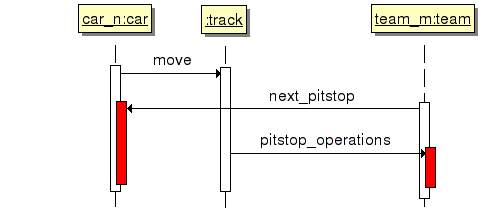
\includegraphics[width=0.8\textwidth]{diagrammi/PitstopDeadlock}
\caption{Possibile situazione di \textit{deadlock}}
\label{fig:pitstopDeadlock}
\end{center}
\end{figure}

La possibile situazione di \textit{deadlock}, qualora il messaggio \texttt{next\_pitstop} fosse inviato in modo sincrono, scaturisce dalla sequenza di messaggi illustrata in figura~\ref{fig:pitstopDeadlock}.

Nello scenario descritto, mentre \car{} sta percorrendo il segmento relativo ai \textit{box} della propria scuderia per effettuare il rifornimento, ovvero invocando il metodo \texttt{track:move}, \team{} tenta di inviare un messaggio \texttt{next\_pitstop} a \car{} rimanendo però bloccato in attesa di una sincronizzazione.

Il metodo \texttt{track:move}, qualora debba simulare una sosta per il rifornimento e calcolare quindi il tempo impiegato per le operazioni, deve invocare il metodo \texttt{team:pitstop\_operations} per ottenere le informazioni su quali operazioni devono essere effettuate durante la sosta. Anche in questo caso la sincronizzazione fallisce e il chiamante rimane bloccato poiché il destinatario del messaggio è ancora bloccato a causa dell'invio del messaggio \texttt{next\_pitstop}.

In questo modo si concretizza una situazione di attesa circolare che porta conseguentemente al \textit{deadlock} precedentemente accennato.

\begin{figure}
\begin{center}
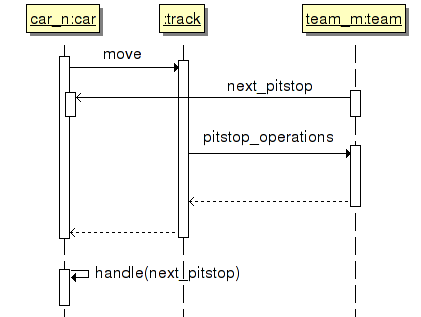
\includegraphics[width=0.7\textwidth]{diagrammi/PitstopSolution}
\caption{Prevenzione dell'attesa circolare}
\label{fig:pitstopSol}
\end{center}
\end{figure}

La soluzione strutturale adottata per evitare questa situazione di attesa circolare è descritta in figura~\ref{fig:pitstopSol}. L'invio del messaggio \texttt{next\_pitstop} è stato reso asincrono per evitare che \team{} rimanga bloccato, come invece accade nello scenario precedente, e sia quindi disponibile alla successiva sincronizzazione causata dalla ricezione del messaggio \texttt{pitstop\_operations}.

Una volta completato lo spostamento l'auto può quindi andare a considerare il messaggio \texttt{next\_pitstop}.

La soluzione appena descritta tuttavia è fonte di un nuovo problema: il fatto che il messaggio \texttt{next\_pitstop} sia inviato in modo asincrono introduce il problema relativo alla freschezza delle informazioni che il messaggio veicola. Supponiamo infatti di avere una conformazione della pista tale per cui appena prima del segmento \texttt{pitstop} di una scuderia vi sia un segmento di tipo \texttt{intermediate} e supponiamo anche che l'auto A di tale scuderia stia percorrendo la \textit{pit lane} per effettuare una sosta.
\`E possibile che si verifichi la seguente sequenza di eventi:
\begin{enumerate}
\item A percorre il segmento \texttt{intermediate} e viene inviata una \texttt{chrono\_notif} a \evdisp{};
\item A percorre il segmento successivo ed effettua la sosta ai \textit{box};
\item la \texttt{chrono\_notif} arriva alla scuderia di A che, in base ai dati ricevuti sullo stato dell'auto (ormai obsoleti a causa del rifornimento), decide, per esempio, di posticipare al giro successivo la sosta ai \textit{box};
\item A riceve il messaggio e obbedisce alla scuderia, rientrando nuovamente ai \textit{box} nel giro successivo ed effettuando molto probabilmente una sosta inutile.
\end{enumerate}

La soluzione che abbiamo adottato per evitare questo genere di incongruenze prevede che \car{} e \team{} mantengano un contatore delle soste effettuate dall'auto fino a quel momento e che \team{} nel messaggio \fun{next\_pitstop} inserisca anche il valore di tale contatore. Di conseguenza, nel momento in cui viene ricevuto il messaggio, l'auto può verificare la freschezza delle informazioni in esso contenute ed eventualmente ignorarlo. I messaggi provenienti dall'utente ovviamente non necessitano di tale contatore poiché sono considerati dall'auto sempre corretti.

\begin{figure}
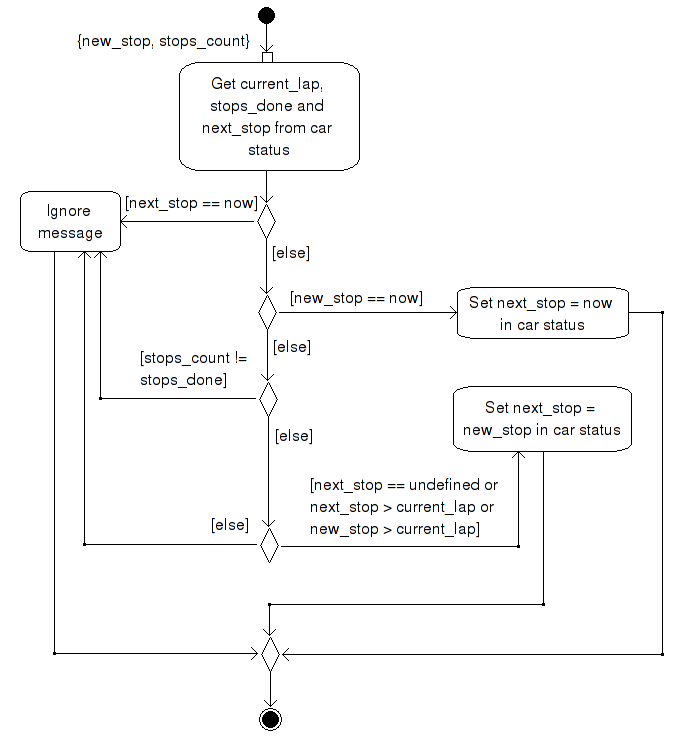
\includegraphics[width=\textwidth]{diagrammi/NextPitstop}
\caption{Algoritmo di \fun{car:set\_next\_pitstop}}
\label{fig:nextPitstop}
\end{figure}

Lato \car{}, l'algoritmo che gestisce l'arrivo di messaggi \fun{next\_pitstop} è quello rappresentato in figura~\ref{fig:nextPitstop}. Il parametro \fun{new\_stop} presente nel messaggio \fun{next\_pitstop} può assumere il valore \fun{now} nel caso in cui la sosta sia imposta dall'utente oppure può essere l'indice del giro in cui effettuare il \textit{pit stop} successivo se la sosta è richiesta dalla logica di \team{}. Come si può notare dalla figura, viene data priorità maggiore alle decisioni dell'utente ignorando i messaggi dei \team{} che potrebbero interferire. Nello stato interno dell'auto, il campo \fun{next\_stop} può assumere i valori \fun{now}, un intero positivo oppure \fun{undefined}. In particolare il valore \fun{undefined} serve ad indicare che non sono state ancora previste soste oppure che l'auto ha appena effettuato un rifornimento e non ha ancora ottenuto direttive dai \team{} o dall'utente.

\subsection{Arrivo}
Un'auto termina la competizione nel momento in cui va a percorrere il segmento successivo al traguardo nell'ultimo giro di gara oppure se si ritira, come descritto in~\ref{sec:percorrenza}. Come si può notare in figura~\ref{fig:move}, nel momento in cui un'auto esce dalla competizione viene invocato il metodo \fun{track:remove\_car} e successivamente il processo termina la propria esecuzione.

Tale metodo serve anche a mantenere aggiornato il contatore delle auto ancora in gara interno alla componente \track{}. Nel momento in cui questo contatore raggiunge il valore zero allora la gara è terminata e \track{} può notificare questo evento al resto del sistema tramite \evdisp{}.

In questo modo le componenti del sistema non più necessarie possono terminare la propria esecuzione, mentre le componenti grafiche possono disabilitare le funzionalità non più disponibili ma restare comunque attive per permettere all'utente di consultare i dati relativi alla simulazione.

\section{Event Dispatcher}
\label{sec:dispatcherImpl}
In questa sezione verrà in primo luogo descritta l'architettura interna della componente \evdisp{}, per poi andarne a motivare le scelte sottostanti.

\evdisp{} è composto da un processo detto \textit{front-end} che ha il compito di ricevere ogni notifica in ingresso e inoltrarla ai processi \textit{back-end} interessati in modo asincrono. Oltre a ciò, il \textit{front-end} deve anche ricevere le richieste di \textit{subscription} e registrare quindi i processi richiedenti presso il corretto \textit{back-end}. Al ricevimento di una notifica un \textit{back-end} provvede ad una eventuale rielaborazione dei dati in essa contenuti per poi inviare il risultato di tale computo ai processi presenti nella sua lista di \textit{subscribers}.

Poiché è stato previsto che una GUI possa registrarsi a simulazione iniziata è necessario che i \textit{back-end} mantengano uno stato interno in modo da poter inviare al \textit{subscriber} che si registra un'immagine parziale dello stato della competizione fino al momento della \textit{subscription}. Successivamente, al richiedente verranno inviate solo le informazioni contenenti i cambiamenti relativi allo stato della competizione e non lo stato stesso in modo da ridurre la quantità di dati inviati. In questo modo non vengono inviati dati ridondanti.

Il diagramma di sequenza in figura~\ref{fig:dispatcher} descrive le operazioni che vengono intraprese da \evdisp{} alla ricezione di una notifica.
Il metodo \fun{filter(msg)} ritorna la lista di \textit{back-end} interessati a ricevere il messaggio \fun{msg} in base al tipo dello stesso.
Il metodo \fun{translate} serve a tradurre un messaggio dal formato utilizzato nella comunicazione \textit{publisher} $\rightarrow$ \evdisp{} al formato usato per la comunicazione \evdisp{} $\rightarrow$ \textit{subscriber}.

\begin{figure}
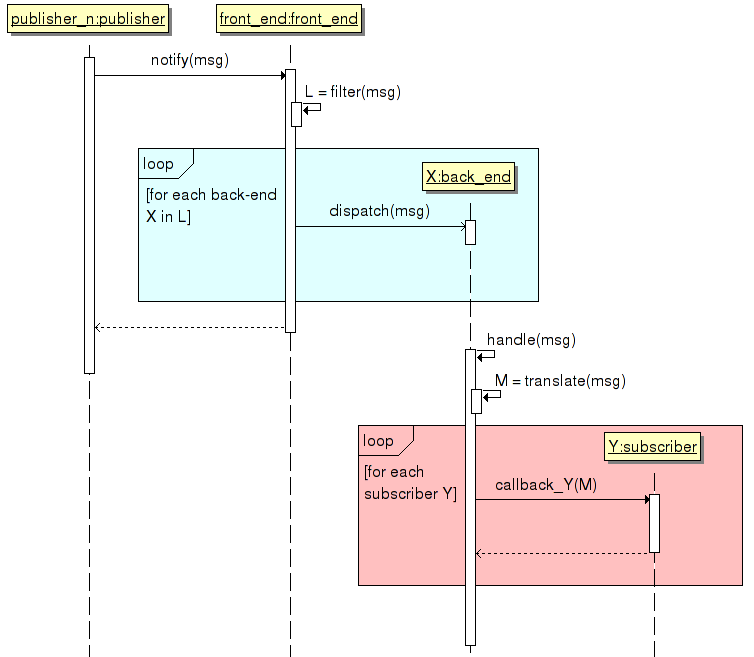
\includegraphics[width=0.9\textwidth]{diagrammi/Dispatcher}
\caption{Propagazione di una notifica tramite \evdisp{}}
\label{fig:dispatcher}
\end{figure}

\subsection*{\textit{Publisher} $\rightarrow$ \textit{front-end}}
Le notifiche relative alla simulazione sono interpretabili in modo corretto solo se considerate nell'ordine in cui vengono emesse.
Per fare un paragone, la visione di un film in cui i fotogrammi vengono permutati casualmente renderebbe la comprensione della trama molto complessa se non impossibile. Allo stesso modo la visione della simulazione che si può ricostruire dalle notifiche di gara differisce a seconda dell'ordine stesso in cui queste vengono considerate.

Un'eccezione a quanto appena detto riguarda le notifiche di configurazione inviate nella fase di bootstrap della simulazione. Queste infatti, per essere utilizzate correttamente, non necessitano di un ordine stretto tra loro ma devono essere tutte valutate prima dell'avvio della gara.

Per il resto del capitolo, nel momento in cui si farà riferimento ai \textit{publishers}, si intenderà il gruppo di processi che inviano notifiche di simulazione al \evdisp{} escludendo quelli che inviano solo notifiche di configurazione. Tale gruppo è quindi composto da \sched{}, \evdisp{} e \car{}.

I \textit{publishers} in realtà eseguono tutti in modo sequenziale poiché ordinati dalla componente \sched{}. Di conseguenza, utilizzando chiamate bloccanti per l'invio delle notifiche da \textit{publisher} a \textit{front-end}, l'ordine di arrivo delle notifiche rimane invariato rispetto l'ordine di invio.

Sarebbe stato comunque possibile raggiungere lo stesso obiettivo utilizzando una comunicazione asincrona, tuttavia, per semplicità si è preferito adottare la soluzione appena descritta. La soluzione asincrona infatti prevedeva di aggiungere ai messaggi un identificatore numerico unico in modo da ottenere un ordinamento totale delle notifiche per poi riordinarle algoritmicamente nel \textit{front-end}. Questo poiché in \Erlang{} l'ordine di invio di messaggi tra due processi può differire dall'ordine di ricezione degli stessi nel caso in cui i processi mittente e destinatario si trovino su nodi differenti.

Risulta quindi evidente che l'utilizzo di comunicazione asincrona in questo caso avrebbe complicato l'implementazione del prototipo, giustificando quindi la scelta di comunicazione sincrona.

\subsection*{\textit{Back-end} $\rightarrow$ \textit{subscriber}}
Le notifiche inviate dai \textit{back-end} devono essere considerate secondo l'ordine di invio dai \textit{subscribers}. Questo perché il primo messaggio inviato dopo la procedura di \textit{subscription} contiene una vista dello stato attuale della simulazione mentre le successive notifiche contengono le variazioni incrementali rispetto allo stato precedente, che hanno senso solo se interpretate nell'ordine corretto. Al fine di avere uno stato consistente il \textit{subscriber} deve perciò ricevere tutte le notifiche e le deve considerare secondo l'ordine di invio.

Assumendo quindi che le notifiche arrivino ai \textit{back-end} nell'ordine corretto, è stato deciso, con un ragionamento analogo a quello esposto nella sezione precedente, di utilizzare l'invio di messaggi sincrono anche per questo tratto del percorso delle notifiche.

Una ulteriore motivazione che ci ha spinto verso l'opzione sincrona è il fatto che la comunicazione, essendo bloccante, fornisce un meccanismo ai \textit{back-end} per rilevare una eventuale disconnessione del destinatario. In questo modo tali componenti possono quindi rimuovere i destinatari non più raggiungibili dalla lista dei loro \textit{subscribers}. Considerando inoltre che il numero di \textit{subscribers} può aumentare e diminuire nel corso della simulazione la soluzione sincrona risulta ancora più vantaggiosa.

\subsection*{\textit{Front-end} $\rightarrow$ \textit{back-end}}
Un'assunzione fatta nella sezione precedente è che le notifiche rimangano ordinate nel passaggio da \textit{front-end} a \textit{back-end}, conseguentemente la soluzione adottata non deve violare questo vincolo.

In questo caso la scelta di comunicazione sincrona avrebbe comportato che, ad ogni notifica inviata, un \textit{publisher} avrebbe dovuto attendere che tale notifica fosse recapitata a tutti i \textit{subscribers} prima di poter continuare la propria esecuzione. Questo perché la notifica sarebbe stata veicolata da sole chiamate bloccanti.

Questa situazione è chiaramente indesiderabile: abbiamo deciso quindi di utilizzare comunicazioni asincrone internamente a \evdisp{}. Il linguaggio utilizzato garantisce che, nel caso di comunicazione asincrona tra processi residenti in uno stesso nodo, l'ordine di ricezione dei messaggi da parte del destinatario è uguale all'ordine di invio dei messaggi da parte del mittente. Grazie a ciò non si è reso necessario un riordino dei messaggi a destinazione, semplificando quindi l'implementazione, ma è stato imposto un vincolo sulla distribuzione dei processi che compongono \evdisp{}.

Il fatto che \textit{front-end} a \textit{back-end} debbano essere su uno stesso nodo non ci è sembrato troppo restrittivo rispetto alla semplificazione in termini di progettazione che l'accettazione di tale vincolo comporta.
